% !TEX root = ../main.tex
\chapter{Documentación de Interfaces (MVP)}

\section{Diagrama de navegación / flujo de pantallas}
La Figura~\ref{fig:diagrama_navegacion} muestra el diagrama de navegación de la aplicación, en el cual los rectángulos corresponden a las pantallas, los círculos a las acciones que el usuario realiza sobre ellas y las flechas al recorrido entre unas y otras. A partir de la lista de tableros el usuario accede a un tablero, donde agrega, edita, une, recarga y elimina tarjetas, y comparte el tablero configurando sus accesos.

\begin{figure}[H]
  \centering
  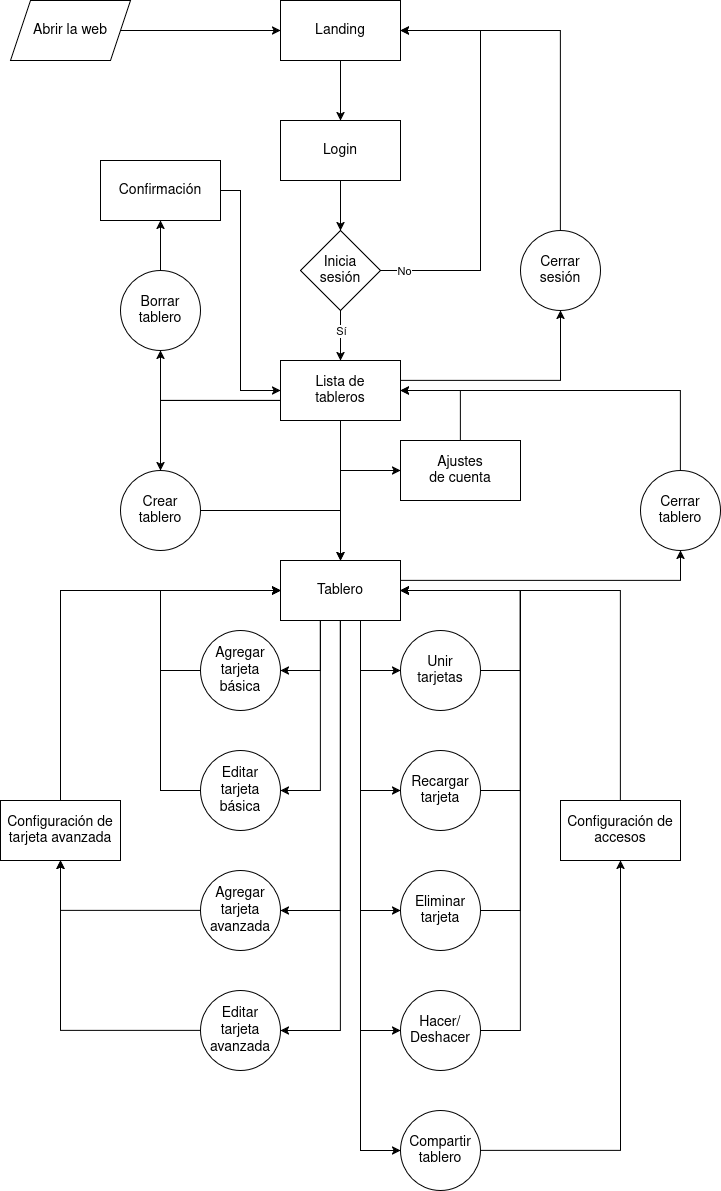
\includegraphics[width=0.82\textwidth]{figuras/fig03.png}
  \caption{Diagrama de Navegación}
  \label{fig:diagrama_navegacion}
\end{figure}